%%%%%%%%%%%%%%%%%%%%%%%%%%%%%%%%%%%%%%%%%%%%%%%%%%%%%%%%%%%%%%%%%%%%%%%%%%%%%%%
% MOTIVATION
%%%%%%%%%%%%%%%%%%%%%%%%%%%%%%%%%%%%%%%%%%%%%%%%%%%%%%%%%%%%%%%%%%%%%%%%%%%%%%%

%%%%%%%%%%%%%%%%%%% 
% COMMON SENSE REASONING TEASER
%%%%%%%%%%%%%%%%%%%
\begin{frame}{Common Sense Reasoning with Natural Logic}
\begin{tabular}{cc}
  \true{Kittens play with yarn} & \false{Kittens play with computers} \\
  \vspace{0.25cm} \\
  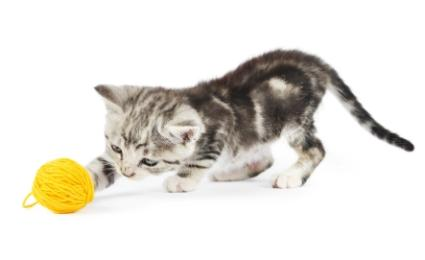
\includegraphics[width=5cm]{../img/yarn-cat.jpg} & \pause 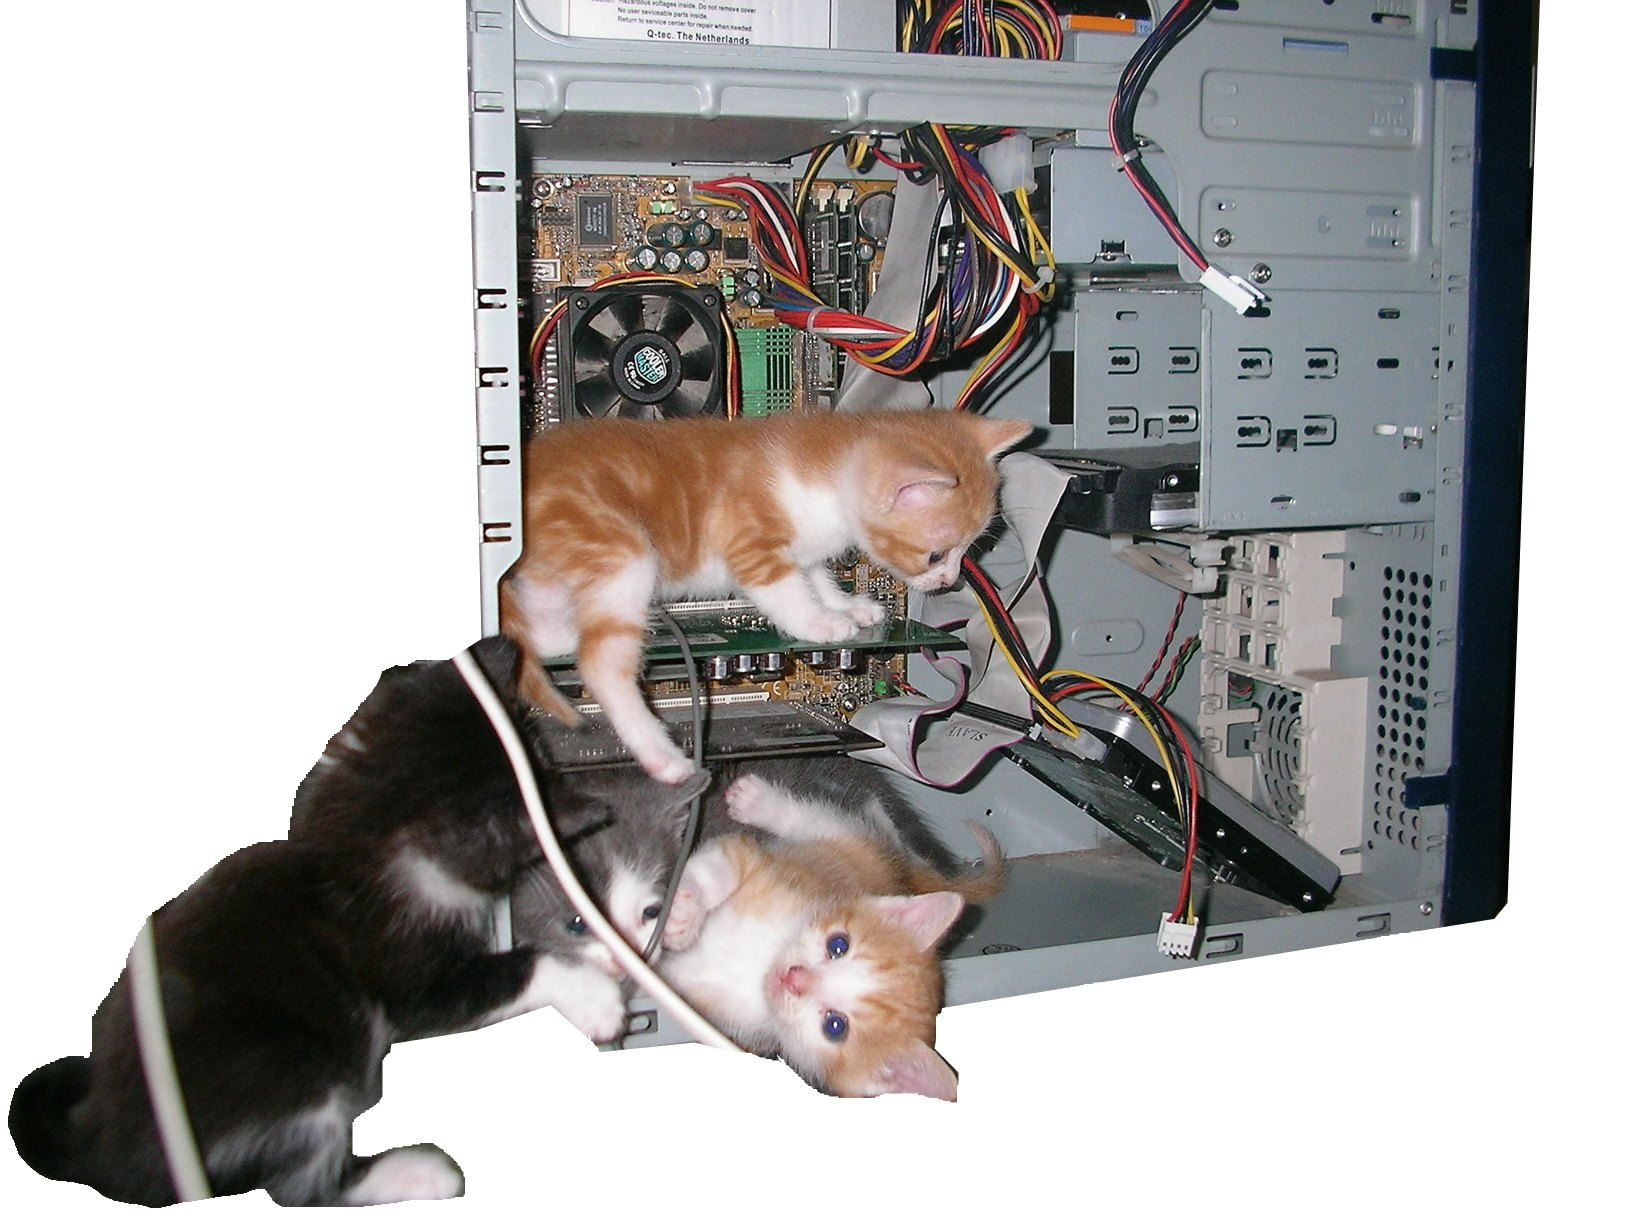
\includegraphics[width=5cm]{../img/computer-cat-cropped.jpg}
\end{tabular}
\end{frame}


%%%%%%%%%%%%%%%%%%% 
% COMMON SENSE REASONING NLP
%%%%%%%%%%%%%%%%%%%
\begin{frame}{Common Sense Reasoning for NLP}
\begin{center}
  \w{The city refused the demonstrators a permit because they feared violence.} \\
  \pause
  \begin{tabular}{l}
    \true{a city fears violence} \\
    \false{demonstrators fear violence}
  \end{tabular}
\end{center}
\pause

\begin{center}
  \w{I ate the cake with a cherry} \hspace{0.25cm} vs. \hspace{0.25cm} \w{I ate the cake with a fork} \\
  \begin{tabular}{l}
    \true{cakes come with cherries} \\
    \false{cakes are eaten using cherries}
  \end{tabular}
\end{center}
\pause

\begin{center}
  \w{Put a sarcastic comment in your talk. That's a great idea.} \\
  \begin{tabular}{l}
    \false{Sarcasm in your talk is a great idea}
  \end{tabular}
\end{center}

\end{frame}

%%%%%%%%%%%%%%%%%%% 
% COMMON SENSE REASONING VISION
%%%%%%%%%%%%%%%%%%%
\begin{frame}{Common Sense Reasoning for Vision}
\begin{tabular}{cc}
  \false{Dogs drive cars} & \true{People drive cars} \\
  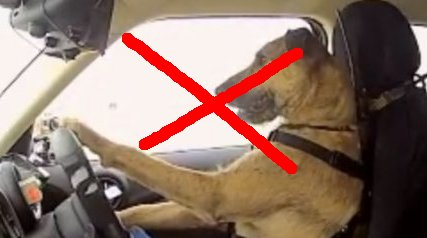
\includegraphics[height=3cm]{../img/dog-driving.jpg} & 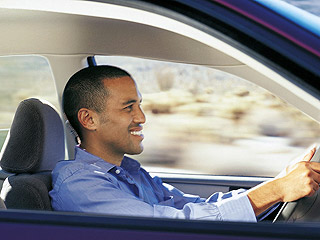
\includegraphics[height=3cm]{../img/person-driving.jpg}  \\
  \vspace{0.0cm} \\
  \pause \false{Baseball is played underwater} & \true{Baseball is played on grass} \\
  
\includegraphics[height=3cm]{../img/baseball-underwater.jpg} & 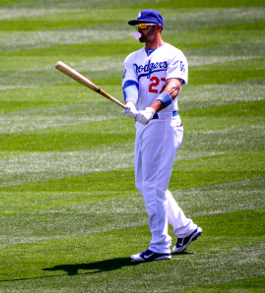
\includegraphics[height=3cm]{../img/baseball-grass.jpg} \\
\end{tabular}
\end{frame}

%%%%%%%%%%%%%%%%%%% 
% COMMON SENSE CURRENTLY
%%%%%%%%%%%%%%%%%%%
\begin{frame}{Prior Work on Common Sense Reasoning}
\hh{Old School AI:} Nuanced reasoning; tiny coverage.
\begin{itemize}
  \item Default reasoning (Reiter 1980; McCarthy 1980).
  \item Theorem proving (e.g., Datalog).
\end{itemize}
\vspace{0.5cm}
\pause

\hh{Textual Entailment:} Rich inference; small data.
\begin{itemize}
  \item RTE Challenges.
  \item Episodic Logic (Schubert, 2002).
\end{itemize}
\vspace{0.5cm}
\pause

\hh{Information Extraction:} Shallow inference, large data.
\begin{itemize}
  \item OpenIE (Yates et al., 2007), NELL (Carlson et al., 2010).
  \item \textit{Extraction} of facts from a large corpus; fuzzy lookup.
%  \pause
%  \item \textbf{Inference doesn't 10x the knowledge base size.}
\end{itemize}
\end{frame}

%%%%%%%%%%%%%%%%%%%% 
%% OpenIE
%%%%%%%%%%%%%%%%%%%%
%\begin{frame}{Open Information Extraction}
%\hh{Mismatch in Evaluation} \\
%\vspace{0.25cm}
%\begin{tabular}{ll}
%  \h{IE Metric} & ``How many facts did I extract'' \\
%  \h{Common Use Case} & ``Is this query in my knowledge base?''
%\end{tabular}
%\end{frame}

%%%%%%%%%%%%%%%%%%% 
% TEASER
%%%%%%%%%%%%%%%%%%%
\begin{frame}{Start with a large knowledge base}
\begin{center}
  \hspace{0.8cm}
  
\includegraphics[height=2.2cm]{../img/database.png}
\end{center}
\end{frame}

\begin{frame}[noframenumbering]{Start with a large knowledge base}
\begin{center}
  \teaserManyPremises
\end{center}
\end{frame}

\begin{frame}[noframenumbering]{Infer new facts...}
\begin{center}
  \teaserBlindInferenceNaturalOrderBlind
\end{center}
\end{frame}

\begin{frame}[noframenumbering]{Infer new facts...}
\begin{center}
  \teaserBlindInferenceNaturalOrder
\end{center}
\pause
\begin{textblock*}{6.0cm}(6.5cm,5cm)
  \textcolor<1-1>{white}{$\uparrow$ Don't want to run inference \\ $~~$ over every fact!}
\end{textblock*}
\pause
\begin{textblock*}{6cm}(5.5cm,7.6cm)
  \textcolor<1-2>{white}{$\leftarrow$ Don't want to store all of these!}
\end{textblock*}
\end{frame}

\begin{frame}[noframenumbering]{Infer new facts...on demand from a query...}
\begin{center}
  \teaserBlindInference
\end{center}
\end{frame}

\begin{frame}[noframenumbering]{...Using text as the meaning representation...}
\begin{center}
  \teaserInference
\end{center}
\end{frame}

\begin{frame}[noframenumbering]{...Without aligning to any particular premise.}
\begin{center}
  \teaserFullDerivation
\end{center}
\end{frame}


%%%%%%%%%%%%%%%%%%%%%%%%%%%%%%%%%%%%%%%%%%%%%%%%%%%%%%%%%%%%%%%%%%%%%%%%%%%%%%%
% INFERENCE
%%%%%%%%%%%%%%%%%%%%%%%%%%%%%%%%%%%%%%%%%%%%%%%%%%%%%%%%%%%%%%%%%%%%%%%%%%%%%%%

%%%%%%%%%%%%%%%%%%% 
% INFERENCE IS SEARCH
%%%%%%%%%%%%%%%%%%%
\begin{frame}{Natural Logic Inference is Search}
\begin{center}
  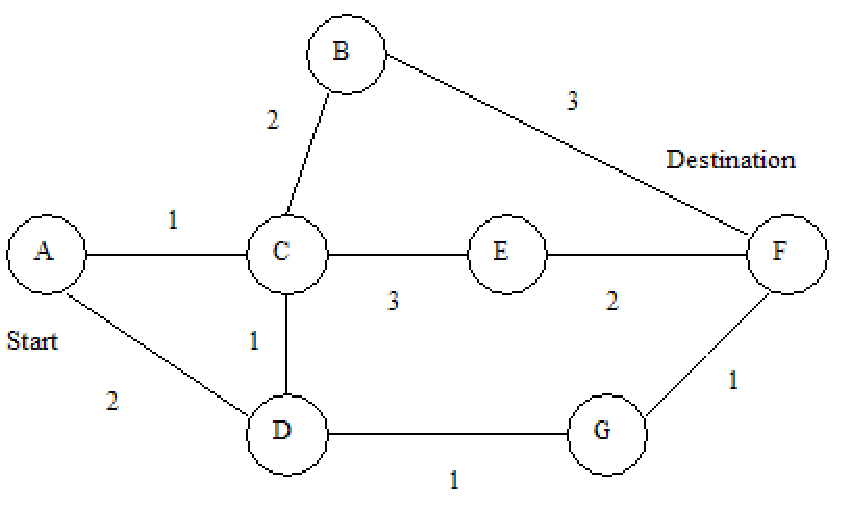
\includegraphics[width=5cm]{../img/dijkstras-graph.pdf}
\end{center}
\begin{tabular}{ll}
  \hh{Nodes} & $($ \w{fact}, truth maintained $\in\{\textrm{true}, \textrm{false}\})$ \\
  & \\
  \pause
  \hh{Start Node} & $($ \w{query fact}, \true{true} $)$ \\
  \hh{End Nodes}  & \w{any known fact} \\
  & \\
  \pause
  \hh{Edges} & Mutations of the current fact \\
  \pause
  \hh{Edge Costs} & How ``wrong'' an inference step is (learned) \\
\end{tabular}
\end{frame}

%%%%%%%%%%%%%%%%%% 
% EXAMPLE SEARCH
%%%%%%%%%%%%%%%%%%
\input exampleSearch.tex

%%%%%%%%%%%%%%%%%%% 
% EDGE TEMPLATES
%%%%%%%%%%%%%%%%%%%
\begin{frame}{Edge Templates}
\begin{center}
  \begin{tabular}{p{0.4\textwidth}p{0.20\textwidth}}
    \multicolumn{1}{c}{\textbf{Template}} & \multicolumn{1}{c}{\textbf{Instance}} \\
    Hypernym & \w{animal} $\rightarrow$ \w{cat} \\
    Hyponym  & \w{cat} $\rightarrow$ \w{animal} \\
    Antonym  & \w{good} $\rightarrow$ \w{bad} \\
    Synonym  & \w{cat} $\rightarrow$ \w{true cat} \\
    & \\
    Add Word  & \w{cat} $\rightarrow$ \w{$\cdot$} \\
    Delete Word  & $\cdot$ $\rightarrow$ \w{cat} \\
    & \\
    Operator Weaken & \w{some} $\rightarrow$ \w{all} \\
    Operator Strengthen & \w{all} $\rightarrow$ \w{some} \\
    Operator Negate & \w{all} $\rightarrow$ \w{no} \\
    Operator Synonym & \w{all} $\rightarrow$ \w{every} \\
    & \\
    Nearest Neighbor  & \w{cat} $\rightarrow$ \w{dog} \\
  \end{tabular}
\end{center}
\end{frame}


%%%%%%%%%%%%%%%%%%% 
% SOFT LOGIC
%%%%%%%%%%%%%%%%%%%
\begin{frame}{``Soft'' Natural Logic}
\hh{Want to make likely (but not certain) inferences}.
\begin{itemize}
  \item Same motivation as Markov Logic, Probabilistic Soft Logic, etc.
  \pause
  \item Each \textit{edge template} has a cost $\theta \geq 0$.
\end{itemize}
\vspace{0.5cm}
\pause

\hh{Detail:} Variation among \textit{edge instances} of a template.
\begin{itemize}
  \item WordNet: \w{cat} $\rightarrow$ \w{feline} \textbf{vs.} \w{cup} $\rightarrow$ \w{container}.
  \item Nearest neighbors distance.
  \item Each \textit{edge instance} has a distance $f$.
\end{itemize}
\vspace{0.5cm}
\pause

\begin{tabular}{ll}
\hh{Cost of an edge is} & $\theta_i \cdot f_i$. \\
\pause
\hh{Cost of a path is} & $\theta \cdot \mathbf{f}$. \pause \\
\multicolumn{2}{l}{\hh{Can learn parameters $\theta$}.}
\end{tabular}

\end{frame}


%%%%%%%%%%%%%%%%%%%%%%%%%%%%%%%%%%%%%%%%%%%%%%%%%%%%%%%%%%%%%%%%%%%%%%%%%%%%%%%
% RESULTS
%%%%%%%%%%%%%%%%%%%%%%%%%%%%%%%%%%%%%%%%%%%%%%%%%%%%%%%%%%%%%%%%%%%%%%%%%%%%%%%

%%%%%%%%%%%%%%%%%%% 
% ConceptNet INTRO
%%%%%%%%%%%%%%%%%%%
\begin{frame}{Experiments}
\hh{ConceptNet:}
\begin{itemize}
  \item A semi-curated collection of common-sense facts. \\
    \vspace{0.1cm}
    \true{not all birds can fly} \\
    \true{noses are used to smell} \\
    \true{nobody wants to die} \\
    \true{music is used for pleasure}
    \vspace{0.1cm}
  \item Negatives: ReVerb extractions marked false by Turkers.
  \item Small (1378 train / 1080 test), but fairly broad coverage.
\end{itemize}
\vspace{0.5cm}
\pause

\hh{Our Knowledge Base:}
\begin{itemize}
  \item 270 million lemmatized Ollie extractions.
\end{itemize}
\end{frame}
  
%%%%%%%%%%%%%%%%%%% 
% ConceptNet RESULTS
%%%%%%%%%%%%%%%%%%%
\begin{frame}{ConceptNet Results}
\hh{Systems}
\begin{itemize}
  \item[] \textbf{Direct Lookup}: Lookup by lemmas.
  \item[] \textbf{NaturalLI}: Our system.
  \pause
  \item[] \textbf{NaturalLI Only}: Use only inference (prohibit exact matches).
\end{itemize}
\pause

\begin{center}
  \begin{tabular}{lcc}
    System             & P     & R    \\
    \hline
    Direct Lookup      & 100.0 & \textbf<5-5>{12.1} \\
    \pause
    NaturalLI Only     & 88.8  & 40.1 \\
    NaturalLI          & 90.6  & \textbf<5-5>{49.1} \\
  \end{tabular}
\end{center}
\pause

\begin{itemize}
  \item 4x improvement in recall.
\end{itemize}
\end{frame}

